% !TeX root = ../../main.tex
\section{Detailed reactor modelling: Toluene nitration (R101)} \label{sec:detailedreactor}

\begin{wraptable}{r}{0.5\linewidth}
\centering
\caption{Reactor overview}
\label{tab:reactoroverview}
\begin{tabular}{@{}lS[table-format=4.2e1]s@{}}
    \toprule
    Parameter                    & {Value} & {Unit}         \\ \midrule
    Overall volumetric flowrate  & 1.32e-4 & \cubic\m\per\s \\
    Number of tubes              & 7       &                \\
    Diameter of each channel     & 0.23    & \m             \\
    Diameter of inner cooling tube & 0.02 & \m \\
    Area of each channel         & 3.14e-2 & \square\m      \\
    Length of reactor            & 4.3     & \m             \\
    Bed voidage                  & 0.277   &                \\
    Mass of H-mordenite required & 59      & \kg            \\
    Mass of inert SiC            & 2092    & \kg            \\
    Volume of liquid in reactor  & 9.24e-1 & \cubic\m       \\
    Total reactor volume         & 2.37    & \cubic\m       \\
    Total pressure drop          & 1.41e-1 & \bar           \\ \bottomrule
\end{tabular}
\end{wraptable}

The nitration of toluene in the heat exchanger reactor (R101) was chosen to be designed in detail for a few reasons. Firstly, the nitration process is most commonly carried out in batch or semi-batch reactors in industry \cite{dugal_nitrobenzene_2005}. Even though there have been incidents of nitration plant explosions such as the Xiangshui plant explosion, the industry has been slow in addressing these safety issues. As part of Nitroma's efforts to enhance the safety of the nitration process by transitioning from batch to continuous process, designing the nitration reactor in detail will allow Nitroma to develop a novel continuous reactor that is inherently safer. Moreover, the nitration reaction is a highly exothermic reaction, so the reactor needs to be robust in controlling the temperature to prevent thermal runaway. The reactor will be optimised to balance safety needs as well as efficient reaction performance. 

Additionally, the industrial nitration reaction typically uses sulfuric acid to protonate the nitric acid to form nitronium ions that are the main nitrating species \cite{sreedhar_scientific_2013}. However, the use of sulfuric acid is not environmentally-friendly as energy is needed to separate the products from the acid and further treatment needs to be done before discharging the sulfuric acid as a wastestream. Therefore, a detailed design of the nitration reactor will allow Nitroma to explore solid catalysts as a substitute, which will be key to Nitroma's goal of being a green company.  

\subsection{Reactor choices}
%"Explain why a particular reactor type was chosen. What were the selection criteria, what other alternatives were considered and why were they ruled out? "
The reactor choices were considered based on several selection criteria, namely, 1) Attrition of catalyst; 2) Hot spot formation; 3) Pressure drop; 4) Heat transfer; 5) Mass transfer; 6) Industrial scalability.
%\begin{enumerate}
    %\item Attrition of catalyst
    %\item Hot spot formation
    %\item Pressure drop
    %\item Heat transfer
    %\item Mass transfer
    %\item Industrial scalability
%\end{enumerate}
A summary of the reactors considered is shown in \cref{tab:reactorchoices}.
\begin{table}[H]
\caption{Summary of reactors considered for toluene nitration (R101)}
\label{tab:reactorchoices}
\begin{tabularx}{\linewidth}{@{}lXX@{}}
\toprule
\textbf{Reactor Candidates}                 & \textbf{Pros}                                                                                               & \textbf{Cons}                                                                                    \\ \midrule
Stirred slurry reactor    & High degree of automation especially temperature control & High attrition of catalyst                                                              \\
\\
Conventional packed-bed reactor    & Ease of operation and fast reaction                                                                & Flow maldistribution and hot spots formation 
\\
\\
Microchannel packed bed reactor    & High heat and mass transfer rate                                                                   & High pressure drop (\textgreater{}40 bar)                                               \\
\\
Coated wall microreactor           & Low pressure drop                                                                                  & Lack of industrial scalability                                                          \\
\\
Plate heat exchanger reactor (HEX) & High heat transfer coefficient                                                                     & Challenging catalyst regeneration process     \\
\\
Shell-and-tube HEX                 & Low pressure drop and high heat transfer coefficient     & Occurrence of fouling                                                                                      \\ \bottomrule
\end{tabularx}
\end{table}

Based on these considerations, a final reactor design of  \textbf{shell-and-tube heat exchanger reactor (HEX) }was chosen as it provides exceptional heat transfer without significant pressure drop. This is particularly important for the nitration reaction as any hotspot formation will lead to a thermal runaway. A high degree of mixing can also be achieved for the usage of different 
%Thinking of creating a table of saying reactor choices//why cannot choose this reactor//
%Several reactors for this reaction were considered for this nitration process including  

The choice of reactors was discussed in detail in \cref{sec:reactorchoices}.

\subsection{Heat of reaction}
To understand the thermal effects of the reaction, the enthalpy of reaction was initially calculated using the enthalpy of formation for each compound participating in the reaction. Data on the standard heat of formation for the compounds were sourced from the NIST website and literature papers.

The enthalpy of reaction was calculated using Hess Law, as shown in the equation below:
\begin{equation}
\label{eq: enthalpyformation}
    \Delta H_{r}^{T} = \Delta H_{f,\mathrm{nitrotoluene}}^{T} + \Delta H_{f,\mathrm{water}}^{T} - \Delta H_{f,\mathrm{toluene}}^{T} - \Delta H_{f,\text{nitric acid}}^{T}
\end{equation}

Since the reaction was carried out at 330K, the enthalpy of reaction was adjusted to the operating temperature by using the heat capacities of the compounds using \cref{eq: enthalpyformation}. The enthalpy of reaction was not further adjusted to capture the effects of pressure since pressure has a negligible effect on the overall enthalpy \cite{liu_nitration_2019}. 

\begin{equation}
    \Delta H_{r}^{330K} = \Delta H_{r}^{\standardstate} + C_p \Delta T
\end{equation}

P-nitrotoluene is an exception since it is a solid at standard state. Therefore, the latent heat of fusion needs to be included when adjusting the enthalpy of reaction to the operating temperature. The summary of the enthalpy of formation for all reactants and products can be found in Appendix \ref{tab:Heat enthalpy table}. The final enthalpy of reaction at 330K is calculated to be -116 kJ/mol. At the specified flowrates of the reactants, the heat duty of the reactor is -63.4 kW.

\subsection{Axial dispersion}
\label{sec:axialdispersion}

\begin{wrapfigure}{R}{0pt}
    % \vspace{-\intextsep}
    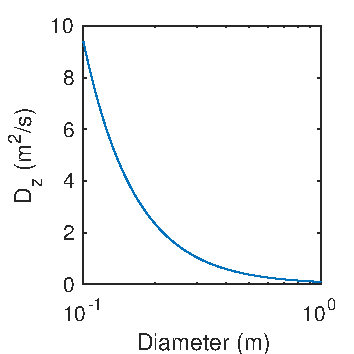
\includegraphics[scale=0.9]{figures/D_z}
    \caption{Dispersion coefficient at various diameter}
    \label{fig:dispersion}
\end{wrapfigure}
\textcite{young_axial_1973} showed that if temperature and concentration distribution (i.e conversion) are important parameters to investigate, then axial dispersion must be taken into account to ensure accurate modelling of flow. A large degree of axial dispersion increases back-mixing in the reactor, which increases the residence time in the reactor and promote undesirable side reactions such as dinitrotoluene or trinitrotoluene. Axial dispersion is a function of the diameter of reacting channels and is independent of the total length. Thus, to minimise the degree of axial dispersion, an optimal diameter needs to be selected. 

The axial dispersion coefficient ($D_z$) can be calculated using the Taylor expression \cite{froment_chemical_2011}: 
\begin{equation}
    D_z=D_{ab}+\frac{(uD)^2}{192D_{ab}}
    \label{eq: axial dispersion coefficient}
\end{equation}
The values of $D_{ab}$ was calculated using the Wilke-Chang correlation.
\begin{equation}
    D_{ab}=\frac{7.4\cdot 10^{-8}(\phi M_2)^{0.5}T}{\mu V_1^{0.6}}
    \label{wilkechang}
\end{equation}
where $D_z$ is the axial dispersion model, $D_{ab}$ is the diffusion coefficient, $u$ is the superficial velocity, $\phi$ is the association parameter which is estimated to be 1 for toluene, $M_2$ is the molecular weight of the solvent which is weighted based on the molar ratio of \ch{HNO3} and water, $V_1$ is the molar volume of toluene at boiling point.

The relationship between axial dispersion coefficient ($D_z$) and diameter was investigated in \cref{fig:dispersion}. Dispersion coefficient decreases exponentially, with \SI{75}{\%} decrease from \SI{1e-1}{\m} to \SI{2e-1}{\m} diameter. Beyond that, the decrease in axial dispersion per unit diameter length plateaus. Although having a larger diameter would decrease axial dispersion further, the drawback of higher CAPEX and larger floor space required does not warrant any further significant increase in channel diameter. A final diameter of \SI{23}{\cm} was selected for each channel, giving an axial dispersion of \SI{1.78}{\metre \squared \per \second}. 

\subsection{Adiabatic temperature profile}

\label{sec:adiabatic}

Nitration is a dangerous process due to its highly exothermic nature. \textcite{di_miceli_raimondi_safety_2015} reported that decomposition of nitric acid begins at \SI{393}{\K}. At temperatures higher than that, thermal decomposition of nitric acid accelerates. This produces a build-up of heat, which increases the rate of reaction, leading to thermal runaway. The reaction also releases poisonous nitrogen oxides as well as other safety risks, which are covered in \cref{sec:NOx}. 

Therefore, to prevent thermal runaway, nitration reactors in industry are typically operated between \si{10} – \SI{50}{°C} below the temperature of runaway reaction \cite{noauthor_lees_2012}. Taking an average temperature between those numbers gives a maximum operating temperature of \SI{30}{\K} below the thermal decomposition of nitric acid of \SI{393}{\K}. Subsequent modelling and safety considerations will aim to keep operating temperature of the nitration process below the safe limit of \SI{363}{\K}. This assumption is in agreement with literature, where most nitration reactions are operated below \SI{373}{\K} as reported by \textcite{chen_experimental_1998}.

As seen in \cref{fig:Adiabatic-without-cooling}, it is infeasible to operate the reactor without controlling its temperature. [insert analysis after the plot is added]

Even with an external cooling jacket to cool down the reactor, the cooling system is insufficient to keep the temperature below \SI{363}{\K}. The temperature quickly spikes above \SI{370}{\K} within the first \SI{0.5}{\m}, and a hotspot can be seen at the radial centre of the pipe. The hotspot will speed up the deactivation of catalyst, but more importantly, it will pose significant safety concerns through the risk of thermal runaway \cite{nguyen_flow_1994}. Therefore, to maintain the safety of the plant, the temperature of the reactor needs to be well-controlled using various methods explained below.

\begin{figure}[h]
    \centering
    
    \begin{subfigure}{0.32\linewidth}
        % 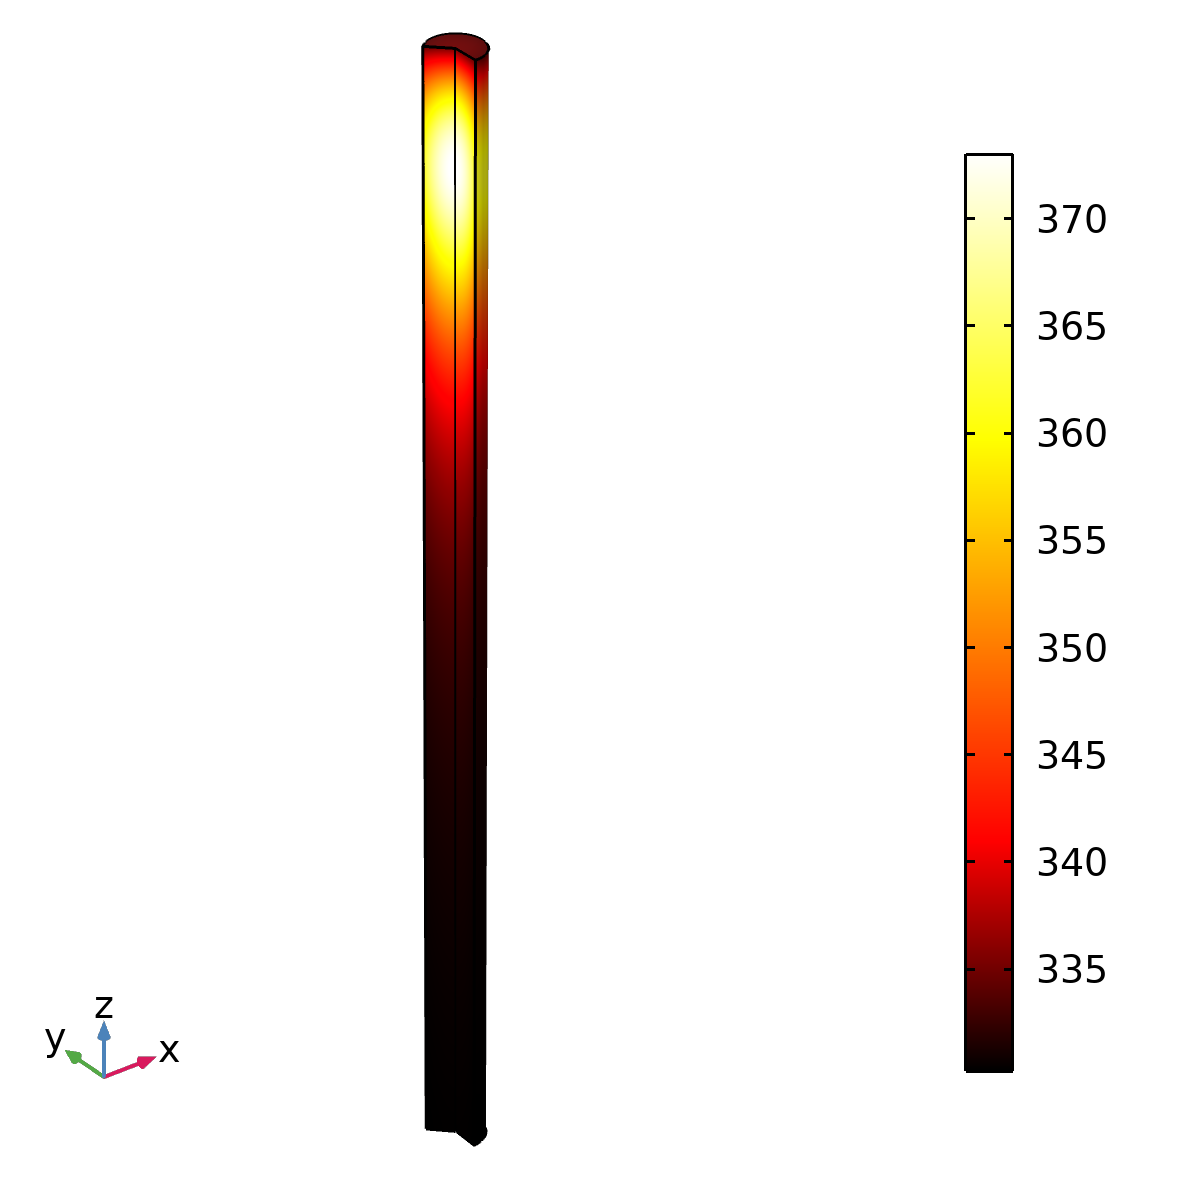
\includegraphics[width=\linewidth]{figures/simple-tube-temperature.png}
        \label{fig:Adiabatic-without-cooling}
        \caption{Adiabatic reactor temperature}
    \end{subfigure}
    \begin{subfigure}{0.32\linewidth}
        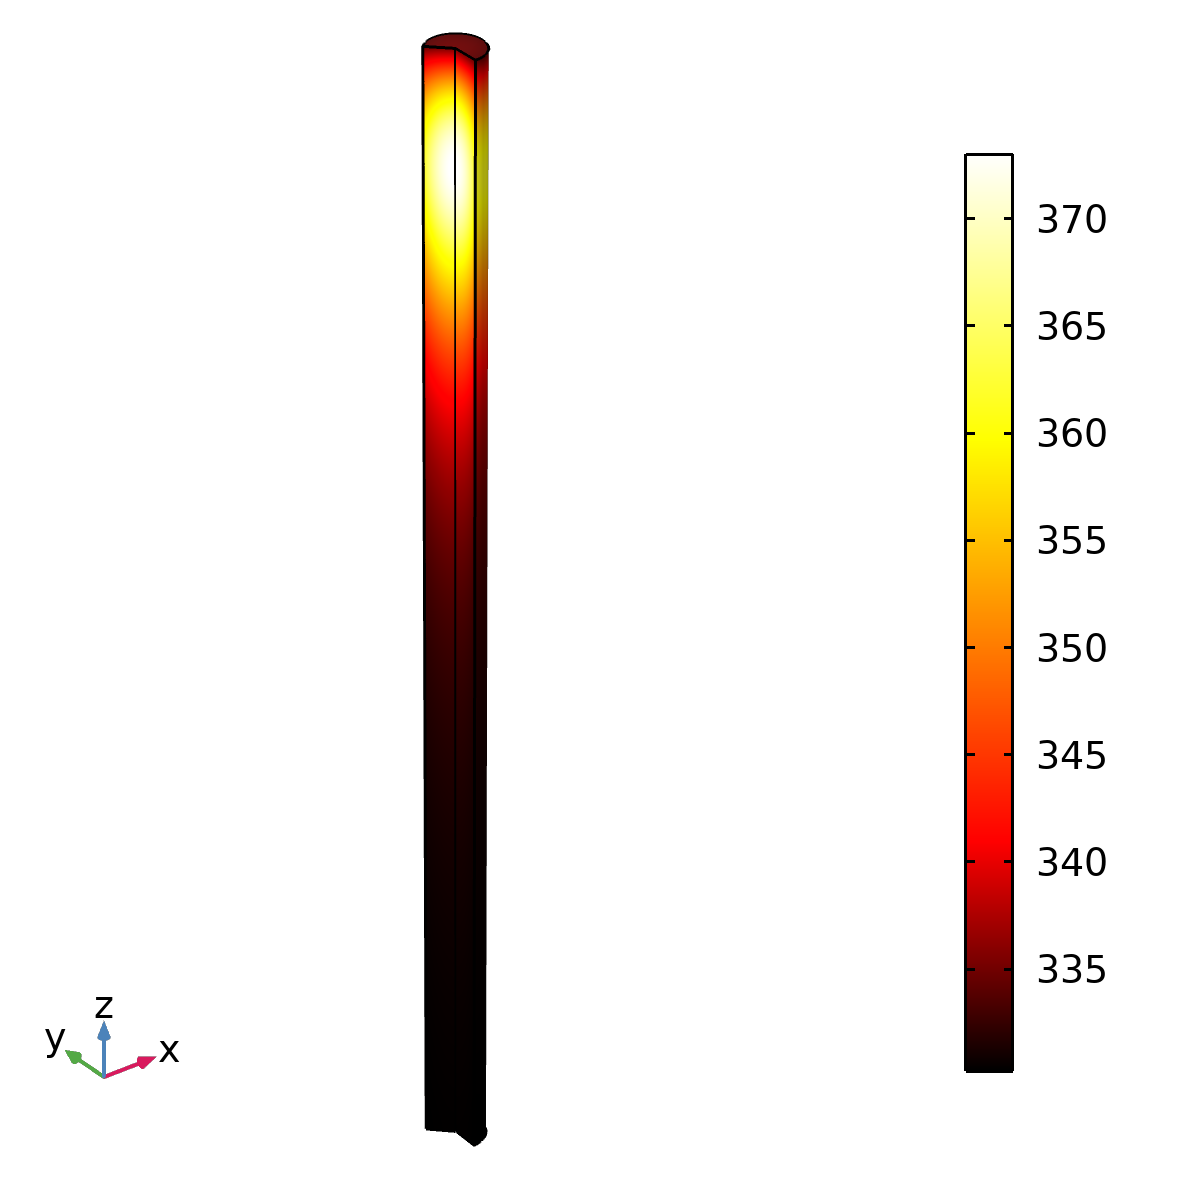
\includegraphics[width=\linewidth]{figures/simple-tube-temperature.png}
        \caption{Temperature with external cooling}
    \end{subfigure}
    

%the other 2 plots should suffice
    %\begin{subfigure}{0.32\linewidth}
        %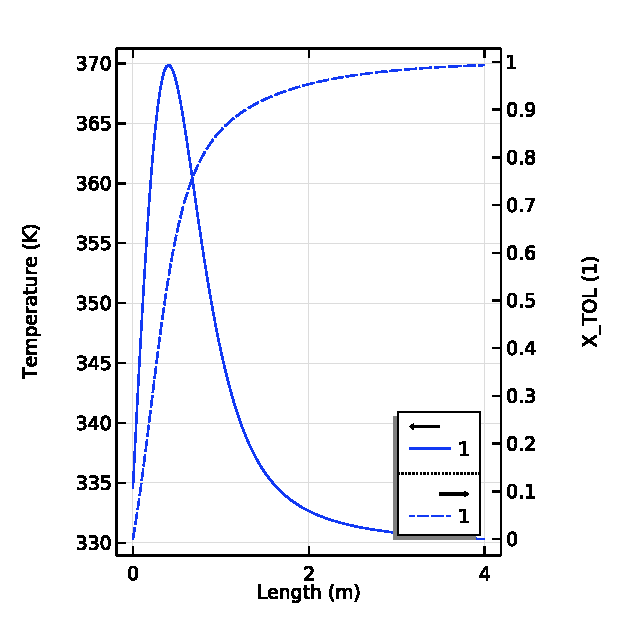
\includegraphics[width=\linewidth]{figures/simple-tube-T-X.eps}
        %\caption{Temperature and conversion profiles}
    %\end{subfigure}

    \caption{Temperature profiles for adiabatic reactor, and with external cooling}
    \label{fig:simple-tube}
\end{figure}

\subsection{Catalyst specification}
\subsubsection{Catalyst support}
Silicon Carbide (SiC) was chosen as the catalyst support owing to its high thermal conductivity (\SI{120}{\W\per\m\per\K} in the bulk, as compared to \SI{3}{\W\per\m\per\K} for H-Mordenite). To immobilise the catalyst, a porous sintered SiC support was selected, with a porosity of 0.30 and thermal conductivity of \SI{40}{\W\per\m\per\K} \cite{jang_thermophysical_2007}. This helps to lower the overall temperature in the reactor by enhancing heat removal from the catalyst surface to the cooling zones \cite{ledoux_silicon_2001}. Although as a result, the rate of reaction and conversion are relatively lower, using SiC keeps the temperature below the critical temperature at which thermal runaway initiates.

Besides, an important feature of the sintered SiC catalyst support is that the tortuosity of the structure promotes homogeneous mixing of the reactants, much like a static mixer \cite{duong-viet_silicon_2016}. As the nitration of toluene is a two-phase reaction, the well-mixed flow increases the interphase contact area, and subsequently increases the rate of reaction. Thus, the reaction can be modelled as a single phase reaction.

Additionally, the nitration reactor would require 270 kg of H-Mordenite catalyst to achieve the desired rate and conversion. However, this could lead to collapse of the catalyst bed due to its weight, which could lead to significant attrition of catalyst and severe pressure drop. The mechanical strength of the SiC support will ensure the catalyst is strongly kept in place when fluid flows through it. The strength of the SiC catalyst support does not decrease over time because SiC forms a silica film when in contact with HNO3 solution, therefore rendering it passive against corrosion \cite{cook_corrosion_2013}. The strength and durability of SiC makes it an ideal material as a catalyst support. The SiC catalyst support used will be fabricated using the partial sintering process with 30 \% porosity before coating it with H-mordenite catalyst.

\subsubsection{Catalyst size}
The H-Mordenite catalyst used in the nitration reaction is deposited on the SiC foam by washcoating. Since the nitration reaction takes place on the surface of the catalyst, it is important to reduce the effect of external and internal diffusional limitation of the reaction depending on the size of the catalyst particle.  

The catalyst particle size was chosen to be 2 µm. At this particle size, the effectiveness factor of the catalyst is $\approx$ 1. An effectiveness factor of $\approx$ 1 suggests that external and internal mass transfer resistances of the catalyst are negligible and the actual rate of reaction is not lowered by mass transfer resistances. The diffusional limitations within the catalyst can also be assumed to be negligible, since the Weisz-Prater criterion of the chosen catalyst size is $\ll$ 1. Detailed calculation can be found in \cref{app:efffactor}.

Typically, catalyst grains, pellets and beads of this diameter would result in a huge pressure drop across the reactor. However, due to the open structure of SiC foam, the pressure drop is significantly reduced \cite{duong-viet_silicon_2016}. In fact, with the same surface area per volume of catalyst bed, catalyst supports have a pressure drop over 10 times smaller than the corresponding packed bed \cite{richardson_properties_2000}. The small catalyst size used in the reaction can therefore reap the benefits of negligible diffusional limitations while avoiding any significant pressure drop.

\subsection{Pressure drop}
%The pressure drop of is a significant consideration in during the selection and modelling of this reactor as the packed-bed reactor shows the 
Even though the pressure drop is expected to be insignificant, efforts were taken to verify the pressure drop of the reactor.

The pressure drop was calculated by using the modified Ergun equation as reported by \textcite{lacroix_pressure_2007}: 
\begin{equation}
    \frac{\Delta p}{L} = \frac{150 \mu (1- \varepsilon)^2 u_0}{\varepsilon^3 d_p^2} + \frac{1.75(1-\varepsilon)\rho u_0^2}{\varepsilon^3 d_p}
    \label{eqn:ergun}
\end{equation}
where foam porosity ($\varepsilon$) is 0.30 from \cite{jang_thermophysical_2007}, $d_p$ is the particle diameter equivalent to the SiC foam structure based only on its mean window size ($a$), using the following formula:
\begin{equation}
d_{p}=\frac{3a[(4 / 3 \pi)(1-\varepsilon)]^{1 / 2}}{2(1-[(4 / 3 \pi)(1-\varepsilon)]^{1 / 2})}
\end{equation}

The pressure drop was calculated to be \SI{0.33}{\bar} which poses no safety risk to the plant. No high pressure pumps will be required, thus saving both OPEX and CAPEX costs.

\subsection{Novel triple concentric tubes}
\label{sec:tripleconctube}
As mentioned in \cref{sec:adiabatic}, it is insufficient to solely rely on the external cooling jacket. Triple concentric tubes heat exchanger (TCTHE) was considered to allow for better temperature control in the reactor. The cooling tube running through the centre of each reactor tube increases the heat exchange area between the reacting fluid and both the inner and outer side of the annulus and also the overall heat transfer coefficient \cite{moya-rico_characterization_2019}. As a result, the enhanced heat transfer rate within the reactor maintains the temperature below \SI{363}{\K} for the reaction, which will be discussed in the final results in Section \ref{finalresults}. Furthermore, a higher heat transfer rate per unit length from the reaction to the cooling fluid in the TCTHE reduces the overall cooling flowrate requirement of the plant. The cooling water is fed into the nitration reactor at \SI{325}{\K} and it will be reused from other parts of the plant to maximise the energy recovery. The summary for reused cooling water stream can be found in \cref{tab:cwtable}.
